% Created by tikzDevice version 0.12 on 2019-04-01 14:59:11
% !TEX encoding = UTF-8 Unicode
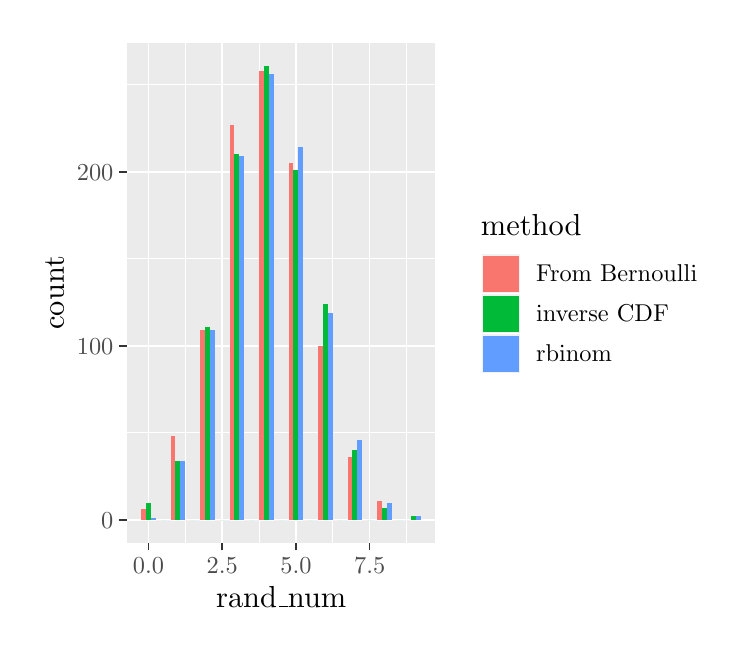
\begin{tikzpicture}[x=1pt,y=1pt]
\definecolor{fillColor}{RGB}{255,255,255}
\path[use as bounding box,fill=fillColor,fill opacity=0.00] (0,0) rectangle (252.94,216.81);
\begin{scope}
\path[clip] (  0.00,  0.00) rectangle (252.94,216.81);
\definecolor{drawColor}{RGB}{255,255,255}
\definecolor{fillColor}{RGB}{255,255,255}

\path[draw=drawColor,line width= 0.6pt,line join=round,line cap=round,fill=fillColor] (  0.00,  0.00) rectangle (252.94,216.81);
\end{scope}
\begin{scope}
\path[clip] ( 35.92, 30.72) rectangle (147.28,211.31);
\definecolor{fillColor}{gray}{0.92}

\path[fill=fillColor] ( 35.92, 30.72) rectangle (147.28,211.31);
\definecolor{drawColor}{RGB}{255,255,255}

\path[draw=drawColor,line width= 0.3pt,line join=round] ( 35.92, 70.38) --
	(147.28, 70.38);

\path[draw=drawColor,line width= 0.3pt,line join=round] ( 35.92,133.28) --
	(147.28,133.28);

\path[draw=drawColor,line width= 0.3pt,line join=round] ( 35.92,196.18) --
	(147.28,196.18);

\path[draw=drawColor,line width= 0.3pt,line join=round] ( 56.96, 30.72) --
	( 56.96,211.31);

\path[draw=drawColor,line width= 0.3pt,line join=round] ( 83.61, 30.72) --
	( 83.61,211.31);

\path[draw=drawColor,line width= 0.3pt,line join=round] (110.25, 30.72) --
	(110.25,211.31);

\path[draw=drawColor,line width= 0.3pt,line join=round] (136.89, 30.72) --
	(136.89,211.31);

\path[draw=drawColor,line width= 0.6pt,line join=round] ( 35.92, 38.93) --
	(147.28, 38.93);

\path[draw=drawColor,line width= 0.6pt,line join=round] ( 35.92,101.83) --
	(147.28,101.83);

\path[draw=drawColor,line width= 0.6pt,line join=round] ( 35.92,164.73) --
	(147.28,164.73);

\path[draw=drawColor,line width= 0.6pt,line join=round] ( 43.64, 30.72) --
	( 43.64,211.31);

\path[draw=drawColor,line width= 0.6pt,line join=round] ( 70.28, 30.72) --
	( 70.28,211.31);

\path[draw=drawColor,line width= 0.6pt,line join=round] ( 96.93, 30.72) --
	( 96.93,211.31);

\path[draw=drawColor,line width= 0.6pt,line join=round] (123.57, 30.72) --
	(123.57,211.31);
\definecolor{fillColor}{RGB}{97,156,255}

\path[fill=fillColor] ( 44.53, 38.93) rectangle ( 46.31, 39.56);
\definecolor{fillColor}{RGB}{0,186,56}

\path[fill=fillColor] ( 42.75, 38.93) rectangle ( 44.53, 45.22);
\definecolor{fillColor}{RGB}{248,118,109}

\path[fill=fillColor] ( 40.98, 38.93) rectangle ( 42.75, 42.71);
\definecolor{fillColor}{RGB}{97,156,255}

\path[fill=fillColor] ( 49.86, 38.93) rectangle ( 51.64, 38.93);
\definecolor{fillColor}{RGB}{0,186,56}

\path[fill=fillColor] ( 48.08, 38.93) rectangle ( 49.86, 38.93);
\definecolor{fillColor}{RGB}{248,118,109}

\path[fill=fillColor] ( 46.31, 38.93) rectangle ( 48.08, 38.93);
\definecolor{fillColor}{RGB}{97,156,255}

\path[fill=fillColor] ( 55.19, 38.93) rectangle ( 56.96, 60.32);
\definecolor{fillColor}{RGB}{0,186,56}

\path[fill=fillColor] ( 53.41, 38.93) rectangle ( 55.19, 60.32);
\definecolor{fillColor}{RGB}{248,118,109}

\path[fill=fillColor] ( 51.64, 38.93) rectangle ( 53.41, 69.13);
\definecolor{fillColor}{RGB}{97,156,255}

\path[fill=fillColor] ( 60.52, 38.93) rectangle ( 62.29, 38.93);
\definecolor{fillColor}{RGB}{0,186,56}

\path[fill=fillColor] ( 58.74, 38.93) rectangle ( 60.52, 38.93);
\definecolor{fillColor}{RGB}{248,118,109}

\path[fill=fillColor] ( 56.96, 38.93) rectangle ( 58.74, 38.93);
\definecolor{fillColor}{RGB}{97,156,255}

\path[fill=fillColor] ( 65.84, 38.93) rectangle ( 67.62,107.49);
\definecolor{fillColor}{RGB}{0,186,56}

\path[fill=fillColor] ( 64.07, 38.93) rectangle ( 65.84,108.75);
\definecolor{fillColor}{RGB}{248,118,109}

\path[fill=fillColor] ( 62.29, 38.93) rectangle ( 64.07,107.49);
\definecolor{fillColor}{RGB}{97,156,255}

\path[fill=fillColor] ( 71.17, 38.93) rectangle ( 72.95, 38.93);
\definecolor{fillColor}{RGB}{0,186,56}

\path[fill=fillColor] ( 69.40, 38.93) rectangle ( 71.17, 38.93);
\definecolor{fillColor}{RGB}{248,118,109}

\path[fill=fillColor] ( 67.62, 38.93) rectangle ( 69.40, 38.93);
\definecolor{fillColor}{RGB}{97,156,255}

\path[fill=fillColor] ( 76.50, 38.93) rectangle ( 78.28,170.39);
\definecolor{fillColor}{RGB}{0,186,56}

\path[fill=fillColor] ( 74.72, 38.93) rectangle ( 76.50,171.02);
\definecolor{fillColor}{RGB}{248,118,109}

\path[fill=fillColor] ( 72.95, 38.93) rectangle ( 74.72,181.72);
\definecolor{fillColor}{RGB}{97,156,255}

\path[fill=fillColor] ( 81.83, 38.93) rectangle ( 83.61, 38.93);
\definecolor{fillColor}{RGB}{0,186,56}

\path[fill=fillColor] ( 80.05, 38.93) rectangle ( 81.83, 38.93);
\definecolor{fillColor}{RGB}{248,118,109}

\path[fill=fillColor] ( 78.28, 38.93) rectangle ( 80.05, 38.93);
\definecolor{fillColor}{RGB}{97,156,255}

\path[fill=fillColor] ( 87.16, 38.93) rectangle ( 88.93,199.96);
\definecolor{fillColor}{RGB}{0,186,56}

\path[fill=fillColor] ( 85.38, 38.93) rectangle ( 87.16,203.10);
\definecolor{fillColor}{RGB}{248,118,109}

\path[fill=fillColor] ( 83.61, 38.93) rectangle ( 85.38,201.21);
\definecolor{fillColor}{RGB}{97,156,255}

\path[fill=fillColor] ( 92.49, 38.93) rectangle ( 94.26, 38.93);
\definecolor{fillColor}{RGB}{0,186,56}

\path[fill=fillColor] ( 90.71, 38.93) rectangle ( 92.49, 38.93);
\definecolor{fillColor}{RGB}{248,118,109}

\path[fill=fillColor] ( 88.93, 38.93) rectangle ( 90.71, 38.93);
\definecolor{fillColor}{RGB}{97,156,255}

\path[fill=fillColor] ( 97.81, 38.93) rectangle ( 99.59,173.54);
\definecolor{fillColor}{RGB}{0,186,56}

\path[fill=fillColor] ( 96.04, 38.93) rectangle ( 97.81,165.36);
\definecolor{fillColor}{RGB}{248,118,109}

\path[fill=fillColor] ( 94.26, 38.93) rectangle ( 96.04,167.88);
\definecolor{fillColor}{RGB}{97,156,255}

\path[fill=fillColor] (103.14, 38.93) rectangle (104.92, 38.93);
\definecolor{fillColor}{RGB}{0,186,56}

\path[fill=fillColor] (101.37, 38.93) rectangle (103.14, 38.93);
\definecolor{fillColor}{RGB}{248,118,109}

\path[fill=fillColor] ( 99.59, 38.93) rectangle (101.37, 38.93);
\definecolor{fillColor}{RGB}{97,156,255}

\path[fill=fillColor] (108.47, 38.93) rectangle (110.25,113.78);
\definecolor{fillColor}{RGB}{0,186,56}

\path[fill=fillColor] (106.69, 38.93) rectangle (108.47,116.93);
\definecolor{fillColor}{RGB}{248,118,109}

\path[fill=fillColor] (104.92, 38.93) rectangle (106.69,101.83);
\definecolor{fillColor}{RGB}{97,156,255}

\path[fill=fillColor] (113.80, 38.93) rectangle (115.57, 38.93);
\definecolor{fillColor}{RGB}{0,186,56}

\path[fill=fillColor] (112.02, 38.93) rectangle (113.80, 38.93);
\definecolor{fillColor}{RGB}{248,118,109}

\path[fill=fillColor] (110.25, 38.93) rectangle (112.02, 38.93);
\definecolor{fillColor}{RGB}{97,156,255}

\path[fill=fillColor] (119.13, 38.93) rectangle (120.90, 67.87);
\definecolor{fillColor}{RGB}{0,186,56}

\path[fill=fillColor] (117.35, 38.93) rectangle (119.13, 64.09);
\definecolor{fillColor}{RGB}{248,118,109}

\path[fill=fillColor] (115.57, 38.93) rectangle (117.35, 61.58);
\definecolor{fillColor}{RGB}{97,156,255}

\path[fill=fillColor] (124.46, 38.93) rectangle (126.23, 38.93);
\definecolor{fillColor}{RGB}{0,186,56}

\path[fill=fillColor] (122.68, 38.93) rectangle (124.46, 38.93);
\definecolor{fillColor}{RGB}{248,118,109}

\path[fill=fillColor] (120.90, 38.93) rectangle (122.68, 38.93);
\definecolor{fillColor}{RGB}{97,156,255}

\path[fill=fillColor] (129.78, 38.93) rectangle (131.56, 45.22);
\definecolor{fillColor}{RGB}{0,186,56}

\path[fill=fillColor] (128.01, 38.93) rectangle (129.78, 43.34);
\definecolor{fillColor}{RGB}{248,118,109}

\path[fill=fillColor] (126.23, 38.93) rectangle (128.01, 45.85);
\definecolor{fillColor}{RGB}{97,156,255}

\path[fill=fillColor] (135.11, 38.93) rectangle (136.89, 38.93);
\definecolor{fillColor}{RGB}{0,186,56}

\path[fill=fillColor] (133.34, 38.93) rectangle (135.11, 38.93);
\definecolor{fillColor}{RGB}{248,118,109}

\path[fill=fillColor] (131.56, 38.93) rectangle (133.34, 38.93);
\definecolor{fillColor}{RGB}{97,156,255}

\path[fill=fillColor] (140.44, 38.93) rectangle (142.22, 40.19);
\definecolor{fillColor}{RGB}{0,186,56}

\path[fill=fillColor] (138.66, 38.93) rectangle (140.44, 40.19);
\definecolor{fillColor}{RGB}{248,118,109}

\path[fill=fillColor] (136.89, 38.93) rectangle (138.66, 38.93);
\end{scope}
\begin{scope}
\path[clip] (  0.00,  0.00) rectangle (252.94,216.81);
\definecolor{drawColor}{gray}{0.30}

\node[text=drawColor,anchor=base east,inner sep=0pt, outer sep=0pt, scale=  0.88] at ( 30.97, 35.90) {0};

\node[text=drawColor,anchor=base east,inner sep=0pt, outer sep=0pt, scale=  0.88] at ( 30.97, 98.80) {100};

\node[text=drawColor,anchor=base east,inner sep=0pt, outer sep=0pt, scale=  0.88] at ( 30.97,161.70) {200};
\end{scope}
\begin{scope}
\path[clip] (  0.00,  0.00) rectangle (252.94,216.81);
\definecolor{drawColor}{gray}{0.20}

\path[draw=drawColor,line width= 0.6pt,line join=round] ( 33.17, 38.93) --
	( 35.92, 38.93);

\path[draw=drawColor,line width= 0.6pt,line join=round] ( 33.17,101.83) --
	( 35.92,101.83);

\path[draw=drawColor,line width= 0.6pt,line join=round] ( 33.17,164.73) --
	( 35.92,164.73);
\end{scope}
\begin{scope}
\path[clip] (  0.00,  0.00) rectangle (252.94,216.81);
\definecolor{drawColor}{gray}{0.20}

\path[draw=drawColor,line width= 0.6pt,line join=round] ( 43.64, 27.97) --
	( 43.64, 30.72);

\path[draw=drawColor,line width= 0.6pt,line join=round] ( 70.28, 27.97) --
	( 70.28, 30.72);

\path[draw=drawColor,line width= 0.6pt,line join=round] ( 96.93, 27.97) --
	( 96.93, 30.72);

\path[draw=drawColor,line width= 0.6pt,line join=round] (123.57, 27.97) --
	(123.57, 30.72);
\end{scope}
\begin{scope}
\path[clip] (  0.00,  0.00) rectangle (252.94,216.81);
\definecolor{drawColor}{gray}{0.30}

\node[text=drawColor,anchor=base,inner sep=0pt, outer sep=0pt, scale=  0.88] at ( 43.64, 19.71) {0.0};

\node[text=drawColor,anchor=base,inner sep=0pt, outer sep=0pt, scale=  0.88] at ( 70.28, 19.71) {2.5};

\node[text=drawColor,anchor=base,inner sep=0pt, outer sep=0pt, scale=  0.88] at ( 96.93, 19.71) {5.0};

\node[text=drawColor,anchor=base,inner sep=0pt, outer sep=0pt, scale=  0.88] at (123.57, 19.71) {7.5};
\end{scope}
\begin{scope}
\path[clip] (  0.00,  0.00) rectangle (252.94,216.81);
\definecolor{drawColor}{RGB}{0,0,0}

\node[text=drawColor,anchor=base,inner sep=0pt, outer sep=0pt, scale=  1.10] at ( 91.60,  7.44) {rand{\_{}}num};
\end{scope}
\begin{scope}
\path[clip] (  0.00,  0.00) rectangle (252.94,216.81);
\definecolor{drawColor}{RGB}{0,0,0}

\node[text=drawColor,rotate= 90.00,anchor=base,inner sep=0pt, outer sep=0pt, scale=  1.10] at ( 13.08,121.02) {count};
\end{scope}
\begin{scope}
\path[clip] (  0.00,  0.00) rectangle (252.94,216.81);
\definecolor{fillColor}{RGB}{255,255,255}

\path[fill=fillColor] (158.28, 86.33) rectangle (247.44,155.71);
\end{scope}
\begin{scope}
\path[clip] (  0.00,  0.00) rectangle (252.94,216.81);
\definecolor{drawColor}{RGB}{0,0,0}

\node[text=drawColor,anchor=base west,inner sep=0pt, outer sep=0pt, scale=  1.10] at (163.78,141.66) {method};
\end{scope}
\begin{scope}
\path[clip] (  0.00,  0.00) rectangle (252.94,216.81);
\definecolor{drawColor}{RGB}{255,255,255}
\definecolor{fillColor}{gray}{0.95}

\path[draw=drawColor,line width= 0.6pt,line join=round,line cap=round,fill=fillColor] (163.78,120.73) rectangle (178.23,135.19);
\end{scope}
\begin{scope}
\path[clip] (  0.00,  0.00) rectangle (252.94,216.81);
\definecolor{fillColor}{RGB}{248,118,109}

\path[fill=fillColor] (164.49,121.45) rectangle (177.52,134.48);
\end{scope}
\begin{scope}
\path[clip] (  0.00,  0.00) rectangle (252.94,216.81);
\definecolor{drawColor}{RGB}{255,255,255}
\definecolor{fillColor}{gray}{0.95}

\path[draw=drawColor,line width= 0.6pt,line join=round,line cap=round,fill=fillColor] (163.78,106.28) rectangle (178.23,120.73);
\end{scope}
\begin{scope}
\path[clip] (  0.00,  0.00) rectangle (252.94,216.81);
\definecolor{fillColor}{RGB}{0,186,56}

\path[fill=fillColor] (164.49,106.99) rectangle (177.52,120.02);
\end{scope}
\begin{scope}
\path[clip] (  0.00,  0.00) rectangle (252.94,216.81);
\definecolor{drawColor}{RGB}{255,255,255}
\definecolor{fillColor}{gray}{0.95}

\path[draw=drawColor,line width= 0.6pt,line join=round,line cap=round,fill=fillColor] (163.78, 91.83) rectangle (178.23,106.28);
\end{scope}
\begin{scope}
\path[clip] (  0.00,  0.00) rectangle (252.94,216.81);
\definecolor{fillColor}{RGB}{97,156,255}

\path[fill=fillColor] (164.49, 92.54) rectangle (177.52,105.57);
\end{scope}
\begin{scope}
\path[clip] (  0.00,  0.00) rectangle (252.94,216.81);
\definecolor{drawColor}{RGB}{0,0,0}

\node[text=drawColor,anchor=base west,inner sep=0pt, outer sep=0pt, scale=  0.88] at (183.73,124.93) {From Bernoulli};
\end{scope}
\begin{scope}
\path[clip] (  0.00,  0.00) rectangle (252.94,216.81);
\definecolor{drawColor}{RGB}{0,0,0}

\node[text=drawColor,anchor=base west,inner sep=0pt, outer sep=0pt, scale=  0.88] at (183.73,110.48) {inverse CDF};
\end{scope}
\begin{scope}
\path[clip] (  0.00,  0.00) rectangle (252.94,216.81);
\definecolor{drawColor}{RGB}{0,0,0}

\node[text=drawColor,anchor=base west,inner sep=0pt, outer sep=0pt, scale=  0.88] at (183.73, 96.02) {rbinom};
\end{scope}
\end{tikzpicture}
